\documentclass[12pt]{article}
\usepackage[utf8]{inputenc}
\usepackage[T1]{fontenc}
\usepackage[italian]{babel}
\usepackage{geometry}
\usepackage[table]{xcolor}
\usepackage{graphicx}
\usepackage{tikz}
\usepackage[export]{adjustbox}


% Configurazione hyperref per link blu sottolineati senza riquadro
\usepackage[colorlinks=true, linkcolor=blue, urlcolor=blue]{hyperref}
\usepackage{ulem} % per sottolineature

% Comando per avere i link blu e sottolineati
\renewcommand\UrlFont{\color{blue}\uline}

% Definizione colori
\definecolor{celeste}{HTML}{AEC6CF}
\definecolor{arancione}{HTML}{FFD699}
\definecolor{grigiochiaro}{HTML}{E8E8E8}

% Margini ridotti per massimizzare lo spazio
\geometry{
  left=1.5cm,
  right=1.5cm,
  top=1cm,
  bottom=1cm
}

% Parametro per dimensione logo (modificabile)
\newcommand{\logosize}{2.5cm}
\newcommand{\signsize}{4cm}

\begin{document}
\pagestyle{empty}

% Immagine a larghezza piena con altezza ridotta
\noindent
\begin{tikzpicture}
  % Immagine delle gole
  \node[anchor=north west, inner sep=0pt] at (0,0) {


  
\includegraphics[width=\textwidth, height=8cm, clip]{foto.jpg}

    
    };
  
  % DECOMMENTARE LE PROSSIME 3 RIGHE PER AGGIUNGERE IL LOGO CAI
  % Logo CAI Juniores sovrapposto in alto a sinistra
   \node[anchor=north west, inner sep=0pt] at (0.3cm,-0.3cm) {
     
\includegraphics[width=\logosize]{../logo_cai_juniores.png}
   };
  
  % Segnale CAI in basso a destra con titolo e data
  \node[anchor=south east, inner sep=0pt] at (\textwidth-0.3cm,-5.7cm) {
    \begin{tikzpicture}
      % Immagine del segnale CAI
      \node[anchor=center, inner sep=0pt] at (0,0) {
        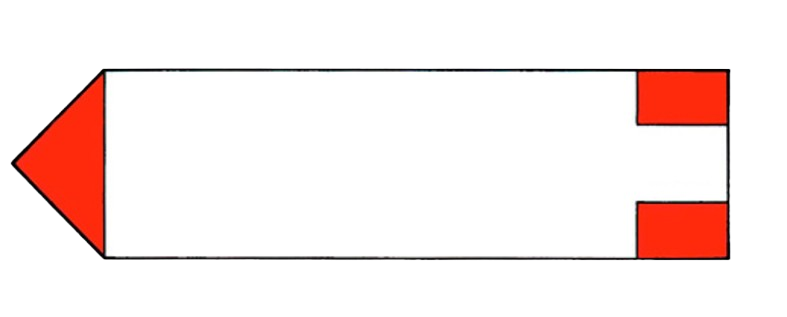
\includegraphics[angle=-10, width=\signsize]{../cai_sign.png}
      };
      % Testo sovrapposto al segnale
      \node[anchor=center,rotate=-10] at (0,-0.15cm) {
        \begin{minipage}{3cm}
          \centering
          \small\textbf{Monte Monte}\\
          \footnotesize\textbf{31/10}
        \end{minipage}
      };
    \end{tikzpicture}
  };
\end{tikzpicture}
  
\vspace{0.5cm}

% APPUNTAMENTO e MEZZO DI TRASPORTO su due righe
\noindent
\colorbox{grigiochiaro}{\parbox{\dimexpr\textwidth-2\fboxsep}{%
\small
\textbf{APPUNTAMENTO:} 31 Ottobre 2025 Roma 6.00.00\\
\textbf{MEZZO DI TRASPORTO:} Auto
}}

\vspace{0.3cm}

% Tabella PROGRAMMA a larghezza piena - prima colonna allargata
\noindent
{\small
\begin{tabular}{|p{3.5cm}|p{\dimexpr\textwidth-3.5cm-4\tabcolsep-3\arrayrulewidth\relax}|}
\hline
\rowcolor{celeste}\multicolumn{2}{|l|}{\textbf{PROGRAMMA: Monte Monte}} \\
\hline
\textbf{Descrizione:} & 
{\footnotesize in pratica questo permetterebbe di fare tutto con Google apps script, con un google form:


1. accompagnatore compila form, volendo lo stesso con cui crea l'uscita (fogli google vari per le prenotazioni etc...)

2. google apps script crea file .tex e lo carica su github (si può fare)

ad esempio potrebbe essere questo file:

https://github.com/aslushnikov/latex-online/blob/master/sample/sample.tex

3. google apps script restituisce questo URL che è il server su cui il file .tex viene compilato online:

https://latexonline.cc/compile?url=https://raw.githubusercontent.com/aslushnikov/latex-online/master/sample/sample.tex


E di fatto quello è già il pdf compilato. Si potrebbe perfino usare quello come link da mettere ovunque, però nel dubbio meglio scaricare il pdf e usare quello.} \\
\hline
\textbf{Dislivello Totale:} & 500 \\
\hline
\textbf{Distanza Totale:} & 5 \\
\hline
\textbf{Difficoltà:} & E \\
\hline
\end{tabular}
}

\vspace{0.3cm}

% Tabella ACCOMPAGNATORI a larghezza piena - prima colonna allargata
\noindent
{\small
\begin{tabular}{|p{3.5cm}|p{\dimexpr\textwidth-3.5cm-4\tabcolsep-3\arrayrulewidth\relax}|}
\hline
\rowcolor{celeste}\textbf{Accompagnatori:} & \cellcolor{arancione}{Arturo} \\ 
\hline
 & Luigi; Arturo; Luigi; Arturo; Luigi  \\
\hline
\end{tabular}
}

\vspace{0.3cm}

% Informazioni finali compatte
\noindent
{\small
\textbf{PORTARE:} \href{https://www.cairoma.it/?page_id=22206}{\textbf{LISTA BASE}} + Nessun materiale in più 

\vspace{0.2cm}
\noindent
\textbf{COSTO:} 5

\vspace{0.2cm}
\noindent
\textbf{ISCRIZIONE:} È necessario essere soci CAI juniores regolarmente iscritti per l'anno in corso o aver pagato l'assicurazione giornaliera.
Iscrizione fino a esaurimento posti: via \href{www.google.com}{\textbf{form}} dall'24/10/2025 alle 5.00.00 al 24/10/2025 alle 5.00.00.
}

\end{document}
